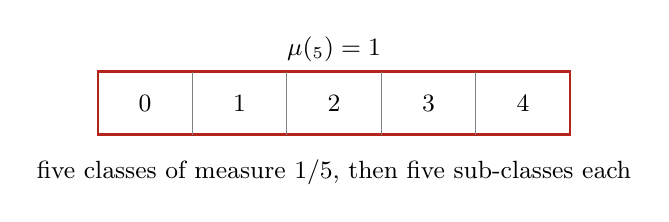
\begin{tikzpicture}[font=\small]
\draw[BrickRed,thick] (0,0) rectangle (6,.8);
\foreach \i in {1,...,4}{\draw[gray] ({6*\i/5},0)--({6*\i/5},.8);}
\foreach \i in {0,...,4}{\node at ({.6+1.2*\i},.4) {$\i$};}
\node[above] at (3,.8) {$\mu(\Z_5)=1$};
\node[below] at (3,-.2) {five classes of measure $1/5$, then five sub-classes each};
\end{tikzpicture}
